\chapter{\statusorange Topics}
\label{chap:topics}

\section{Introduction}

% conclusions from chapter 5:
% two motivations:
% The first one, is to find in which topics propaganda varies mostly across the political spectrum. There may be some topics where the discussion is not using a lot of propaganda techniques to drive the reader in a certain direction, or where the usage may not be very distinctive (e.g., when talking about sports, Left and Right persuasion may be quite difficult to tell apart).
% With an analysis of the topics, we can find the ones where the detected propaganda differs the most, and therefore where we can try to recognise automatically more easily the political leaning of a news article by using the propaganda features.

% % Motivation 2
% And another strong motivation to analyse the topics is to try to locate where the current approach to propaganda detection might have some issues in being accurate.
% % Find topics where propaganda detection might have some problems
% We will perform this analysis and try to find insights that could lead to the development of future propaganda detection resources (e.g., datasets) that are less subject to the imbalance problems that we found in this chapter.



% what

In our last chapter, we concluded with the need to analyse the topics of the articles for two main reasons:

\begin{enumerate}
    \item finding the topics where propaganda varies mostly across the political spectrum. There may be some topics where the discussion is not using a lot of propaganda techniques to drive the reader in a certain direction, or where the usage may not be very distinctive (e.g., when talking about sports, Left and Right persuasion may be quite difficult to tell apart). With an analysis of the topics, we can find the ones where the detected propaganda differs the most, and therefore where we can try to recognise automatically more easily the political leaning of a news article by using the propaganda features.
    \item analyse the topics is to try to locate where the current approach to propaganda detection might have some issues in being accurate. We will perform this analysis and try to find insights that could lead to the development of future propaganda detection resources (e.g., datasets).
\end{enumerate}

This chapter introduces \emph{Topic} as the last ingredient of our analysis.

Hypothesis: some topics have highly distinguishable propaganda, some topics not.
This hypothesis is supported by the work of~\cite{garimella2018quantifying,treuillier2022being} that state that some topics have more polarizing effects because they present higher or lower levels of controversy.
And with this chapter we aim to analyse if this controversy is manifesting through the usage of language of the articles themselves.

%https://hal.archives-ouvertes.fr/hal-03681454/file/umap22adjunct-63.pdf “Given that the topics discussed in the news do not all have the same polarizing effect – they present higher or lower levels of controversy [29] → Kiran Garimella, Gianmarco De Francisci Morales, Aristides Gionis, and Michael Mathioudakis. 2018. Quantifying controversy on social media. ACM Transactions on Social Computing 1, 1 (2018), 1–27


% why
Why?



% RQ

RQs:
\begin{itemize}
    % \item RQ1: How can we optimise the definition of the topic in order to have enough details? 
    % \item RQ2: How does the topic (at different granularities) change across political leaning on a parallel news corpus?
    \item RQ1: How does the detected propaganda change across the topics?
    \item RQ2: How does the detected propaganda change across topics and leanings?
    \item RQ3: How does the topic, combined with the propaganda features, affect the classification of leaning?
    % \item RQ6: Can we find some topics where propaganda detection is not working as expected?
\end{itemize}

% % How
% How?

% How this relates to other chapters


% structure (similar to chap 4 and 5):
% - new ingredient: topic
% - combination with previous ingredients

% findings
findings
\todo{findings}

The structure of this chapter is the following. First, in Section~\ref{sec:top}
methodology in the next section, then each of the experiments that target the research questions, then discussions and conclusions


% two documents:

% Experiment 7: contains an analysis of different ways of extracting/using topics on my dataset. Here I show some breakdown by topic using some topics annotations in the dataset (AllSides topics), and also with the values from TextRazor (CoarseTopics, Fine-grained topics, but not yet using the hierarchical MediaTopics)

% Expanding the topics of AllSides: also includes the analysis of MediaTopics (IPTC)


% For the code, I have two parts:
% https://github.com/MartinoMensio/textrazor-bulk-annotate which can be used to annotate a dataset.
% attached the code from a private repository (bcanalytics) which contains some functions to handle the taxonomy (file src/textrazor.py ) and to plot the sunburst diagrams (file experiments/text\_razor.ipynb)

\section{Methodology}
\label{sec:topic_method}

Being our main goal to understand how propaganda varies across topics and leanings, we first need to decompose it as we are introducing a new factor in our analysis.
For this reason, this chapter first starts analysing different methods and definitions of topic on their own, and gradually combines it with leaning and propaganda. The result is that we have similar experiments that only differ in the different factors included.
We group the experiments in two broad types:
\begin{enumerate}
    \item experiments to select and refine the topic detection methodology: we compare different techniques, and we discuss what we need from the topic; 
    \item experiments that combine topic and propaganda: here we analyse and answer the Research Questions listed before.
\end{enumerate}

Across the experiments of this whole chapter, we use the same methodology, that we describe here.

\begin{figure}[!htbp]
    \centering
    \resizebox{\textwidth}{!}{
    \trimbox{2cm 1cm 2cm 1cm}{% \digraph{abc}{
%   rankdir=LR;
%   a -> b -> c;
% }


% \digraph{structs} {
%     node [shape=record];
%      rankdir=LR
%     struct1 [label="<f0> left|<f1> mid dle|<f2> right"];
%     struct2 [label="<f0> one|<f1> two"];
%     struct3 [label="hello\gvnewline world |{ b |{c|<here> d|e}| f}| g | h"];
%     struct1:f1 -> struct2:f0;
%     struct1:f2 -> struct3:here;
% }

% \resizebox{\textwidth}{!}{
\digraph{chap6} {
    rankdir="LR";
    node [shape=record];
    annotation [label="annotations"];
    a1 [label="topic"];
    a2 [label="leaning"];
    a3 [label="propaganda"];
    combination [label="combination"]
    e_type1 [label="refine topic methodology"]
    e_type2 [label="answer RQs"]
    e1 [label="topic at different granularities"]
    e2 [label="topic across leanings"]
    e3 [label="propaganda across topics\gvnewline RQ1"]
    e4 [label="propaganda across topics+leanings\gvnewline RQ2"]
    e5 [label="CLF (topic, propaganda)  leaning \gvnewline RQ3"]
    
    annotation -> a1;
    annotation -> a2;
    annotation -> a3;
    a1 -> combination;
    a2 -> combination;
    % a3 -> combination;
    a3 -> e_type2;
    combination -> e_type1;
    combination -> e_type2;
    e_type1 -> e1;
    e_type1 -> e2;
    e_type2 -> e3;
    e_type2 -> e4;
    e_type2 -> e5;
}
% }
    }}
    \caption{Methodology of Chapter 6}
    \label{fig:methodology_mindmap_chapter6}
\end{figure}


\subsection{Dataset annotation}

For the experiments, we take, as in the previous chapter, the \texttt{baly} dataset.

We make use of annotations that cover different dimensions:
- Propaganda: as in the previous chapters, words and techniques
- Leaning: from the dataset itself (L/C/R), as in previous chapter
- Topic analysis: provided by TextRazor, coarse topics, topics, IPTC topics (explain in detail what they are)


\subsubsection{Topic annotation}
We use for the experiments of this chapter different topic annotations. As we discussed in Chapter~\ref{sec:lit_topics_computation}, there are several methods that can be used, but in this chapter we focus on the results given by TextRazor.
TextRazor gives topics in different ways:

\begin{enumerate}
    \item Coarse topics
    \item fine-grained topics
    \item IPTC media topics: hierarchical
    \item entities with their types.
\end{enumerate}

We use them and compare in Sections~\ref{sec:topic_topic_granularities} and~\ref{sec:topics_topics_leaning}.

\subsection{Processing and combining the annotations}

Having the annotations related to three different dimensions (propaganda/leaning/topic) we compare them to understand what varies between the different topics, combining them gradually with the other two dimensions (propaganda and leaning).



\subsection{Linking the experiments together}
% How each of the following experiments is linked together

For each of the experiments, we combine differently the annotations and analyse their relationship. For experiments 1-4, we observe the differences when applying different partitioning of the dataset (based on the chosen annotations). For experiment 5, we instead use the annotations of the topic to break down the results of the political leaning classifier of the previous chapter.

% description of each experiment
TODO: type 1 and type 2, then hierarchically all the experiments

Topic analysis at different granularities:
coarse topics, fine-grained, hierarchical. We need hierarchical topic that can go into detail because high-level topics are very broad and distributions are not very meaningful. We need to take a closer look at the details, but as well to understand where these detailed topics stand in the larger picture. (RQ1)

Topic analysis across political spectrum:
Coarse topics are very similar across political spectrum
Fine-grained topics are slightly different (quantity, terms). Which ones? They express the choice of details that we discussed in chapter 3

PROPAGANDA and Topic: only considering hierarchical topics.
Which topics contain more detected propaganda?
How detected propaganda varies across topics? 

Propaganda and Topic and Leaning:
Which topics have propaganda that differs the most across the spectrum? (Quantities of techniques/terms/) Measured with the correlation of (propaganda features) between Left and Right.
Do some of the findings clash with the “knowledge of the context”/”what should happen”? These topics may be the problem for propaganda detection
Political Leaning Classifier with Propaganda features: adding Topic
Breakdown of F1 measure across topics. Not train/test but just looking at the models trained in the previous chapter and seeing which topics were more easy/difficult to predict. We cannot train a classifier with 50/100 articles.



% \section{Topic analysis}
% \label{sec:topic_topic}

% Why: understand which practical definition of topic is better for our analysis. Granularity, type, ...

% How: First we recall the definition of topic that we gave in Chapter~\ref{sec:lit_topics} and the computational approaches that are mostly used.

% \subsection{Topic definition}
% \label{sec:topic_topic_def}

% What it is:
% - categories / groups 
% - refer to chapter 2 briefly

% How it relates to concepts described in this thesis:
% - headlines, clusters
% - topic and anti-topic layers/words: refer to Chapter~\ref{ssec:lit_layers_of_info}

% \subsection{Computational Approaches}
% \label{sec:topic_topic_computation}

% \todo{Everything here goes in chapter 2}

% Explain here different tools/methods that provide topics/entities

% We have approaches that try to determine the topics without having external knowledge, and approaches that instead an existing taxonomy/list of topics and try to map the input documents to them.

% \subsubsection{LDA topics}

% One of the most common methods to extract topics is to ``automatically detecting them" from the corpus.
% The idea is to learn from the data and by selecting a specific number of output topics, we get them.
% Problem: difficult to extract labels

% The problem of assigning labels: can we really tell what is different about the groups?
% Need to know beforehand how many topics we want in output.
% TODO

% Topic identification is a method for identifying hidden subjects in enormous amounts of text1. It can help you find common themes or keywords that represent the main ideas of a document or a collection of documents. For example, if you have a set of news articles, you can use topic identification to find out what are the most discussed topics among them.

% One of the techniques for topic identification is called Latent Dirichlet Allocation (LDA)12. It is a statistical model that assumes that each document is composed of a mixture of topics, and each topic is composed of a distribution of words. LDA can learn these topics and words from the data without any prior knowledge or labels. LDA can be implemented using Python’s Gensim package1, which provides various tools for natural language processing.

% LDA is a type of topic modeling that uses a latent Dirichlet allocation approach12. Topic modeling is a form of unsupervised learning that can be used for exploring unstructured text data by inferring the relationships that exist between the words in a set of documents23.

% LDA assumes that each document is composed of a mixture of topics, and each topic is composed of a distribution of words13. LDA can discover topics that are hidden (latent) in a set of text documents by inferring possible topics based on the words in the documents34. LDA uses a generative probabilistic model and Dirichlet distributions to achieve this4.

% Another technique for topic identification is called bag-of-words2. It is a simple way to represent text data as a collection of words and their frequencies. Bag-of-words ignores the order and structure of sentences, but it can capture some basic information about the content and vocabulary of a document. Bag-of-words can be used with simple NLP models such as TF-IDF or Naive Bayes to identify topics from texts.


% \subsubsection{Entity Annotators}
% DBPedia spotlight: entity annotation is not very good. It struggles to recognise all the entities in the articles (proof?) → DISCARDED
% BLINK (Facebook): huge (30GB models to fit on RAM), not running on my laptop. On server: no NVIDIA drivers (wants GPU) → DISCARDED
% Spacy-entity-linker https://github.com/egerber/spaCy-entity-linker/ . Not very widely used. → DISCARDED

% Then from entities, need ways to derive the topics by navigating knowledge bases (wikidata in most cases)

% \subsubsection{TextRazor}
% TextRazor: seems more accurate, industrial, FreeBase taxonomy. Each entity is annotated with wikidata id and a list of FreeBase types. Also provides topics and fine-grained topics

% benchmarks? check that it is better than other tools
% % Regarding the validation of TextRazor, I am not aware of a benchmark done to check if it is better than other tools. It was suggested by Harith to use it, and I find that the data it provides is generally quite good (for topics and entities). But this is qualitative, I didn’t do a benchmark or looked up for benchmarks. The assumption was that it’s a commercial product and it should be good.
% some papers that claim to do benchmarks:
% http://giusepperizzo.github.io/publications/Rizzo\_Erp-LREC2014.pdf for the entities
% https://www.linkedin.com/pulse/google-nli-kill-market-linguistic-apis-review-yuri-kitin/ mentioning that TextRazor is useful because it links to Wikipedia/DBPedia

% TextRazor is the only one that provides already hierarchical topics, the other ones always give topics that are not hierarchical or can be made hierarchical with external knowledge (e.g. using DBPedia to navigate broader topics).

% What it provides




\section{Topic at different granularities}
\label{sec:topic_topic_granularities}
% ONLY TOPIC
Why: understand which practical definition of topic is better for our analysis. Granularity, type, ...

% How: First we recall the definition of topic that we gave in Chapter~\ref{sec:lit_topics} and the computational approaches that are mostly used.

% analysis of baly dataset at different granularities

% RQ1 (NO): How can we optimise the definition of the topic in order to have enough details? 

We start with the definition of topics that is contained in the Baly dataset, and then we use the different topic types that we get from TextRazor, starting with simple ones to get to the more complex.

\subsection{Custom topics (AllSides)}

The first topic definition that we apply is the ones that comes directly from the \texttt{baly} dataset.

Pro: defined by the authors, by hand
Cons: hierarchically disomogeneous, highly imbalanced

Original topics
The dataset is provided together with topic labels but they have a big problem: they are annotated with labels that have very different granularities.
108 topic labels
Most frequent topics: elections, politics (very general), white house, immigration, healthcare
Least frequent topics: dea, capital punishment and death penalty, fda, south corea
Labels are not uniform:
In granularity: e.g., elections vs politics, one is a subtopic of the other
In aspect: e.g. geography (south corea, africa, china, russia) vs more generic and traversal (food, privacy, healthcare, …)

\begin{figure}[!htbp]
    \centering
    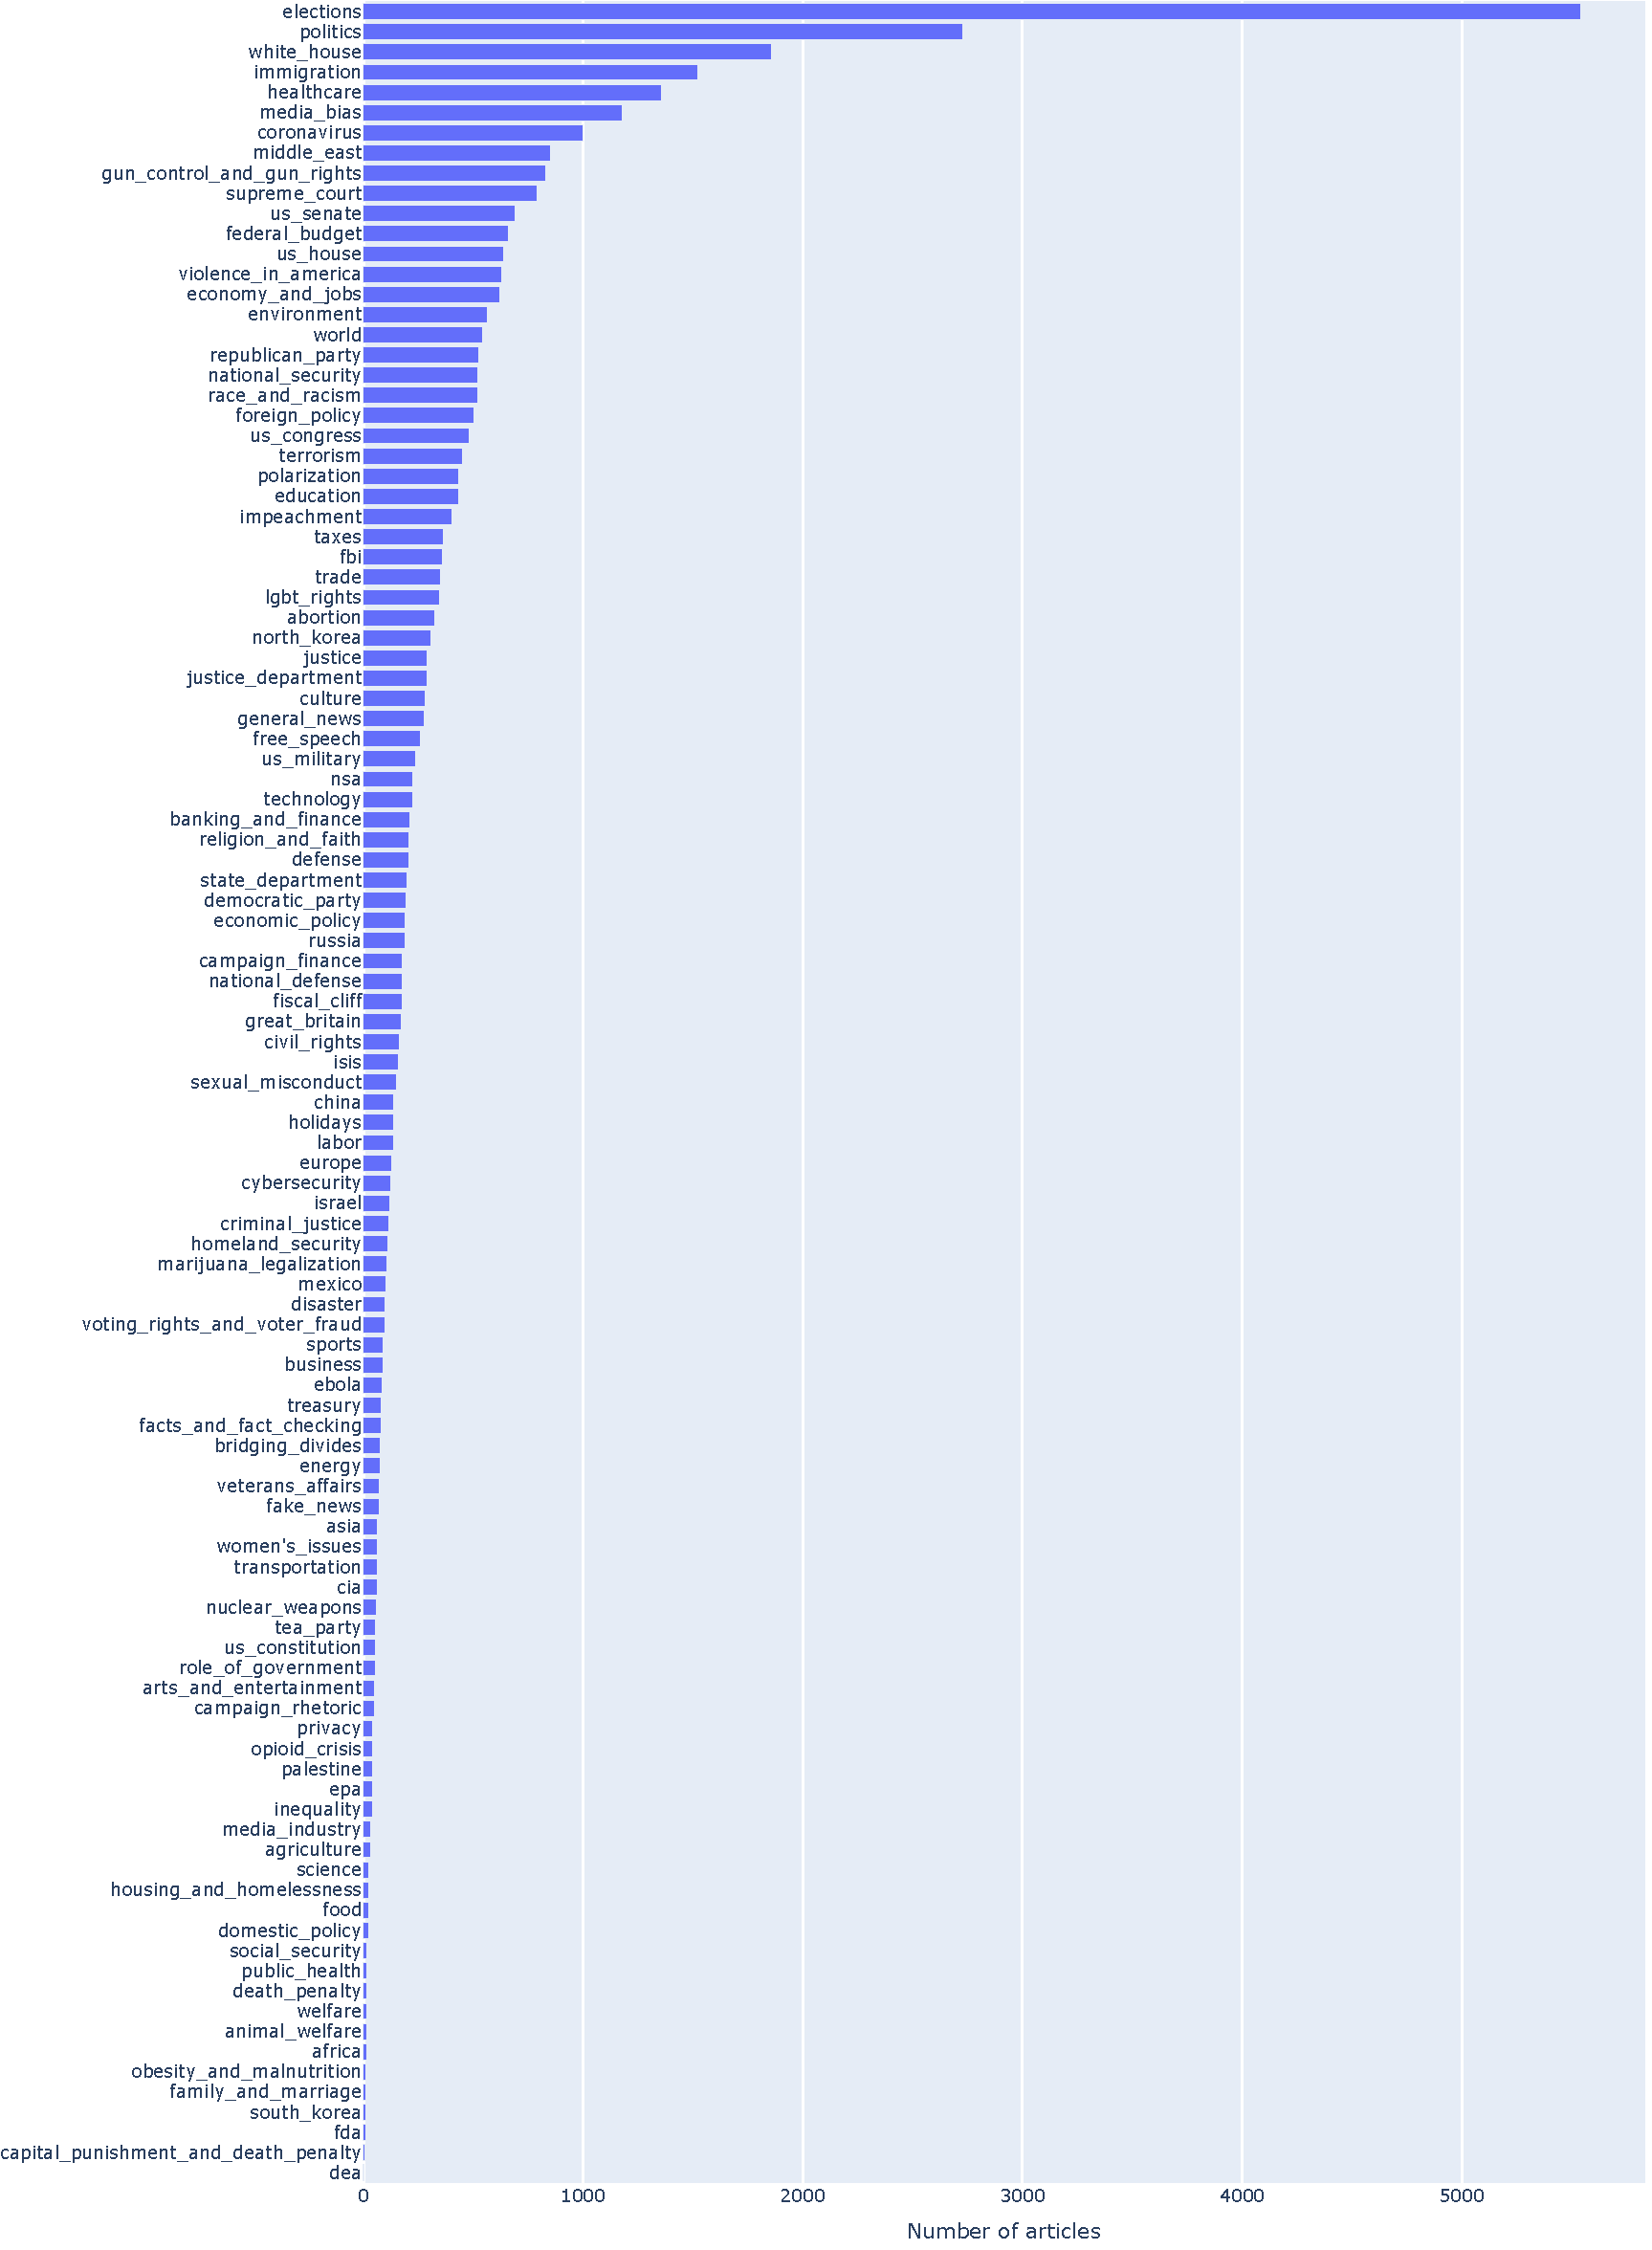
\includegraphics[width=\linewidth]{figures/baly_original_topics.pdf}
    \caption{Original topics of \texttt{Baly} dataset}
    \label{fig:baly_original_topics}
\end{figure}

These topic labels are given by the AllSides team with an unknown criteria, and the above shows how diverse and not-uniformed they are.


\subsection{Coarse Topics}

In this section we take into consideration the TextRazor coarseTopics annotations. TextRazor is a commercial API that allows to analyse topics, entities and to perform other NLP-related tasks (e.g. classify documents, …).
Regarding the topics, it provides coarseTopics, which are 17 very high-level topics (Belief, Business, Culture, Education, Health, Language, Law, Leisure, Mathematics, Nature, Politics, Science, Sports, Technology, Violence, Weather).
Each document is assigned with the top 5/6 matching coarseTopic, each one with a relevance score which ranges in [0,1]. Those scores don’t sum to 1. Each document is assigned to multiple topic, not a single one.

\subsubsection{Most relevant topic Only}

Most relevant topic only
Each article only associated with the first (most important) topic. The topics from the second onwards are discarded.

\begin{figure}[!htbp]
    \centering
    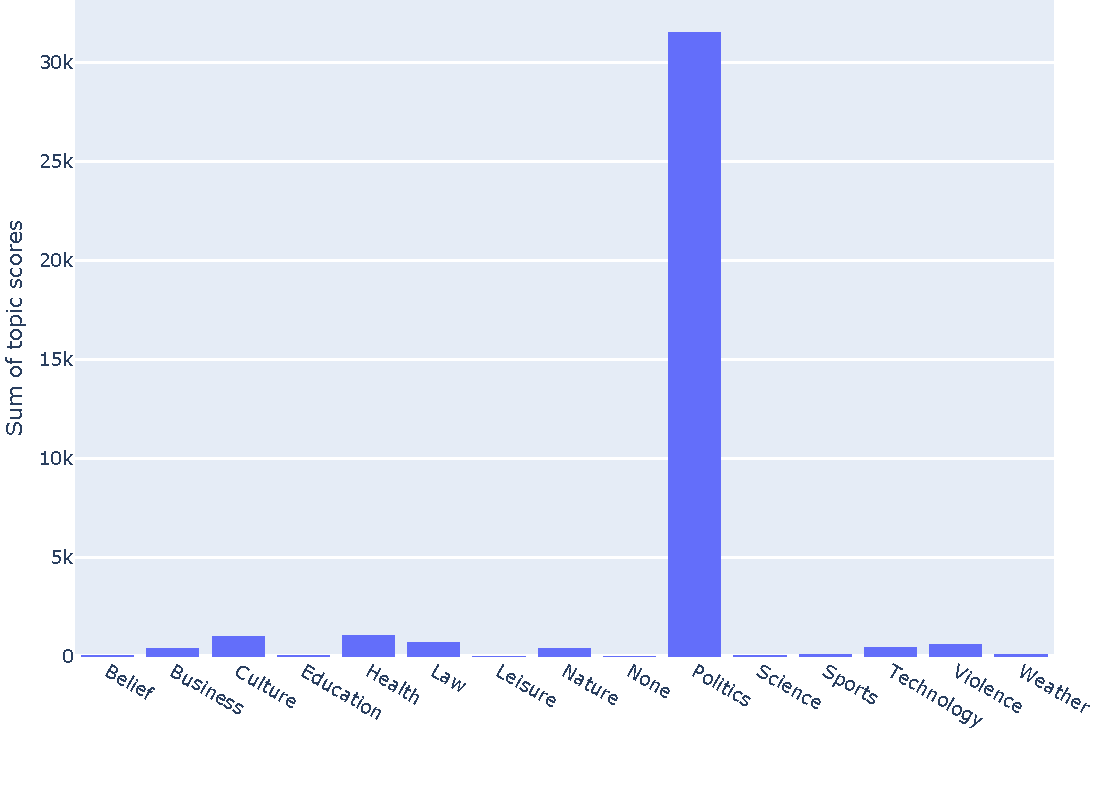
\includegraphics[width=\linewidth]{figures/baly_coarse_first.pdf}
    \caption{Coarse Topics most relevant of \texttt{Baly} dataset}
    \label{fig:baly_coarse_first}
\end{figure}

This shows that the dataset is highly unbalanced on Politics. This makes this topic annotation highly unusable.

\subsubsection{Weighted (multi-topic)}
If we consider each of the 5/6 topic for each article and not only the first one, we get the following distribution:

\begin{figure}[!htbp]
    \centering
    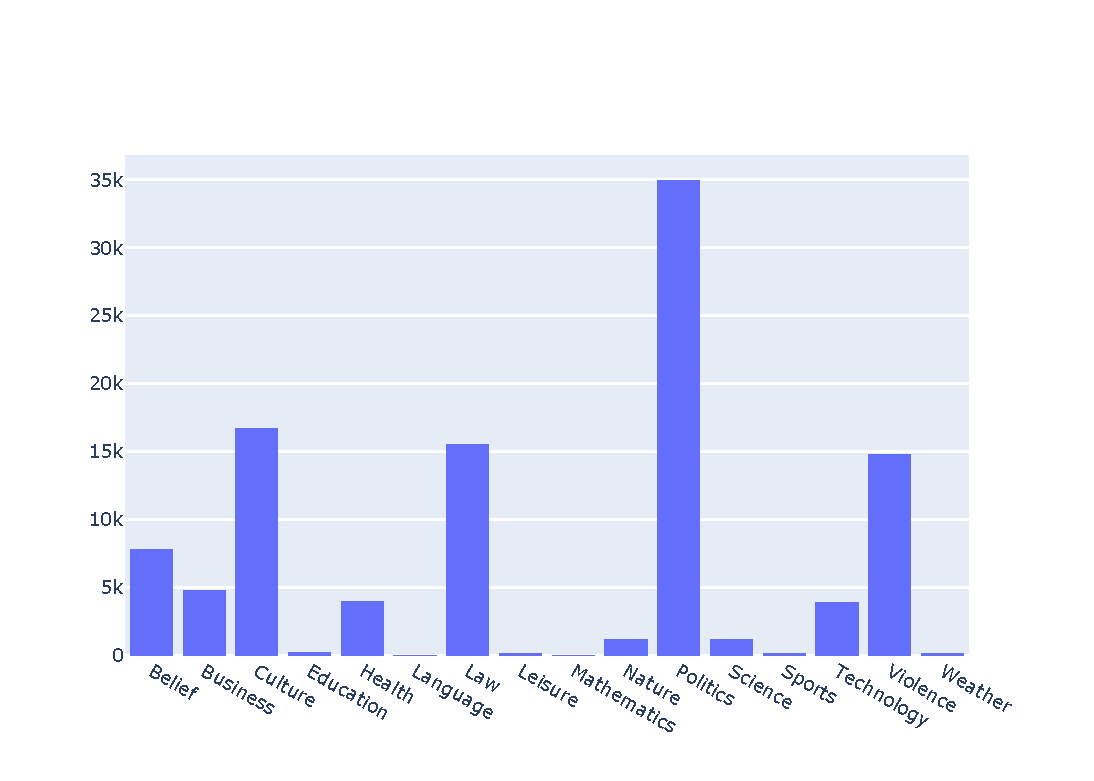
\includegraphics[width=\linewidth]{figures/baly_coarse_weighted.pdf}
    \caption{Coarse Topics weighted of \texttt{Baly} dataset}
    \label{fig:baly_coarse_weighted}
\end{figure}

We can see that the distribution is slightly unbalanced towards politics, then culture, law and violence. This looks like the topics are not too unbalanced, but we have to remember that we would like to have a single document to be categorised only with one topic, and this is not the case.


What this means:
the coarseTopics are not enough granular to be able to split the data in significant groups (across political spectrum)
Being the percentages across political leaning quite similar, this confirms the underlying grouping of triples of articles in the dataset (expected)


\subsection{Fine-Grained Topics}

Baly dataset: 99941 fine-grained topics overall
Example:
TODO FIGURE MONGO TOPICS

annotated only at the article level (not possible to align with propaganda techniques)
Many distinct: 98.504
At this point maybe we could directly use the entities which have a word-level annotation 

They have wikidata\_id → can see their type and do something smart

find some of them that are specific of a political leaning? 

\subsubsection{How to reduce/aggregate?}

Reduction to different granularities of topics:
Wikidata IDs → wikidata embeddings? (too difficult, also to explain the features and analysis / explanation)
Wikidata ← → link to IPTC topics (offered by IPTC, handmade by them)
For each entity, navigate its triples to find IPTC topics. Relationships of type:
Instance\_of
Subclass\_of
???
In theory, every type of relationship is important: e.g. “Trump Wall” Q61989464 is “named after” Donald Trump 

Why not LDA-topics?
Difficult to label?

Trying to find topics that are not so tight
https://en.wikipedia.org/wiki/Wikipedia:Contents/Categories 
This number of topics is too high. How to climb a bit up the topic tree in Wikidata?
wikidataId → entity. From the entity navigate the relationships instance\_of and subclass\_of. But also other relationships could be useful?
From WikiLink → wikipedia page. From the page navigate the categories (recursively) to climb up the categories tree (in reality it’s a Graph) of wikipedia \url{https://en.wikipedia.org/wiki/Special:CategoryTree?target=Category\%3APolitics&mode=all&namespaces=&title=Special%3ACategoryTree}
In both ways, the upper categories are many for each node, and it’s quite difficult to get a clean taxonomy.
Previous works:
https://www.academia.edu/download/30772075/ponzetto\_slides.pdf cleaning up relationships to extract pages+categories taxonomy.
https://aclanthology.org/P14-1089.pdf WiBi taxonomy → http://wibitaxonomy.org/ dead http://ceur-ws.org/Vol-1272/paper\_81.pdf https://aclanthology.org/P14-1089.pdf https://www.diag.uniroma1.it/navigli/pubs/IJCAI\_2009\_Ponzetto\_Navigli.pdf 
https://dl-acm-org.libezproxy.open.ac.uk/doi/abs/10.1145/3308558.3313519 for fictional domain, cleaning up category graph for fictional domains

Backlinks? What are they?

Wikipedia categories github experiment? https://github.com/wasiahmad/mining\_wikipedia/tree/master/WikiNomy 



\subsubsection{With IPTC}
So let’s take all the relationships and navigate some hops until an IPTC topic comes up (termination).
Feature building: decay with the number of hops the weight (exponentially? 1, 0.5, 0.25, …) of each entity.
Table of entities (quite many distinct), with filter on number of appearances

\subsubsection{Without IPTC}

We can just take a look at the fine-grained topics:
Minimum support filter (to reduce features) or select top-k topics

Option with linked entities:
Don’t lose a lot of fine-grained topics/entities which don’t have enough support
Consider them with the related entities in KB
How to do this: 
Navigate hops from each entity (decay weight)





\subsection{Derived from Entity types}

Freebase Taxonomy revised by TextRazor

entity propaganda feature computation
For each entity, compute the total/average propaganda techniques that co-occur in the same sentence %by each political leaning.
E.g.: “Donald Trump” used a lot of times with “Doubt” % from the Left leaning.

Interesting direction:
With Entity linking (provided by TextRazor) it is possible to find common attributes of the entities that make them targets of %Left/Right 
propaganda. E.g., a category of people as repeated target of Propaganda

\subsubsection{filter the entities types}

Using all the entities is too much.

Option 1: choose the types that will be mostly framed differently by Left/Center/Right (related to politics and sensitive topics e.g. Wikipedia list/ Allsides List
Option 2: automatically discover the types that are featured more differently from L/C/R in the training dataset


Analysis of the types listed in FreeBase
TextRazor: https://www.textrazor.com/blog/2015/10/freebase-type-deduction-with-data.html they took freebase and are continuing to update it.
FreeBase build taxonomy: path-like. Let’s build the tree from the path pieces (e.g. /Location/Country is a child of /Location)
Interesting types: religion, military, law, business, organisation, government, location/country, people (how to justify?)

Freebase Taxonomy (revised by TextRazor): https://drive.google.com/file/d/145CpFSFA0\_kuzvNt4z\_H1F2nKi-9-YyF/view?usp=sharing 
Entities types appearing on the headlines dataset: https://drive.google.com/file/d/166fz78O\_xKesnCQ\_hDGiLSH5jk8WdV86/view?usp=sharing 



\subsection{IPTC Topics}

Problem: very difficult to group fine-grained topics into more wide ones
Solution: IPTC NewsCodes Media Topics schema https://cv.iptc.org/newscodes/mediatopic/
It’s a taxonomy (5-levels categories)
TextRazor also provides mediatopic if request is performed with appropriate parameters.

https://iptc.org/news/wikidata/ 
TreeView: \url{https://show.newscodes.org/index.html?newscodes=medtop&lang=en-GB&startTo=Show}

https://cv.iptc.org/newscodes/mediatopic/
17 top-level terms
5-level taxonomy
Each article is annotated with up to 10 topics (with a weight from 0.0 to 1.0), for each one of them we can see the upper topics in the hierarchy
Top-level mediatopics in the Baly dataset


Expecially developed for news
Hierarchical


Problem: topic is very unbalanced on this dataset (everything about “politics”)
Breaking down with respect to topic, is not helpful to find differences between L/C/R if the topic splitting is very unbalanced and very generic.
When breaking a dataset of news articles we want to have the possibility to break down the topic enough to see differences. (e.g. In which topics the Left/Right are enough different in how they use propaganda?)



IPTC mediatopics
TextRazor gives in response 10 mediatopics for each article, each one with a score

\subsubsection{Most relevant topic only}
All levels, only pick first one (most important)

TODO figure


Problem: only politics and government.
How to solve: when multiple labels are given, avoid the most broad/common ones. E.g.: politics:1.0, politics>elections: 0.85 → choose elections

What if, instead of trying dirty ways to select only one topic for each article, we keep the multi-topic annotations?
- Each article instead of having only one topic, is a distribution over a set of topics
- In the downstream tasks we can use this distribution as the topic description (why should it be only one topic?)
- If we proceed in this way, we should also do the same analysis with the standard topic distribution (not mediatopics)


\subsubsection{Weighted full taxonomy}
Each article can belong to multiple categories.

\begin{figure}[!htbp]
    \centering
    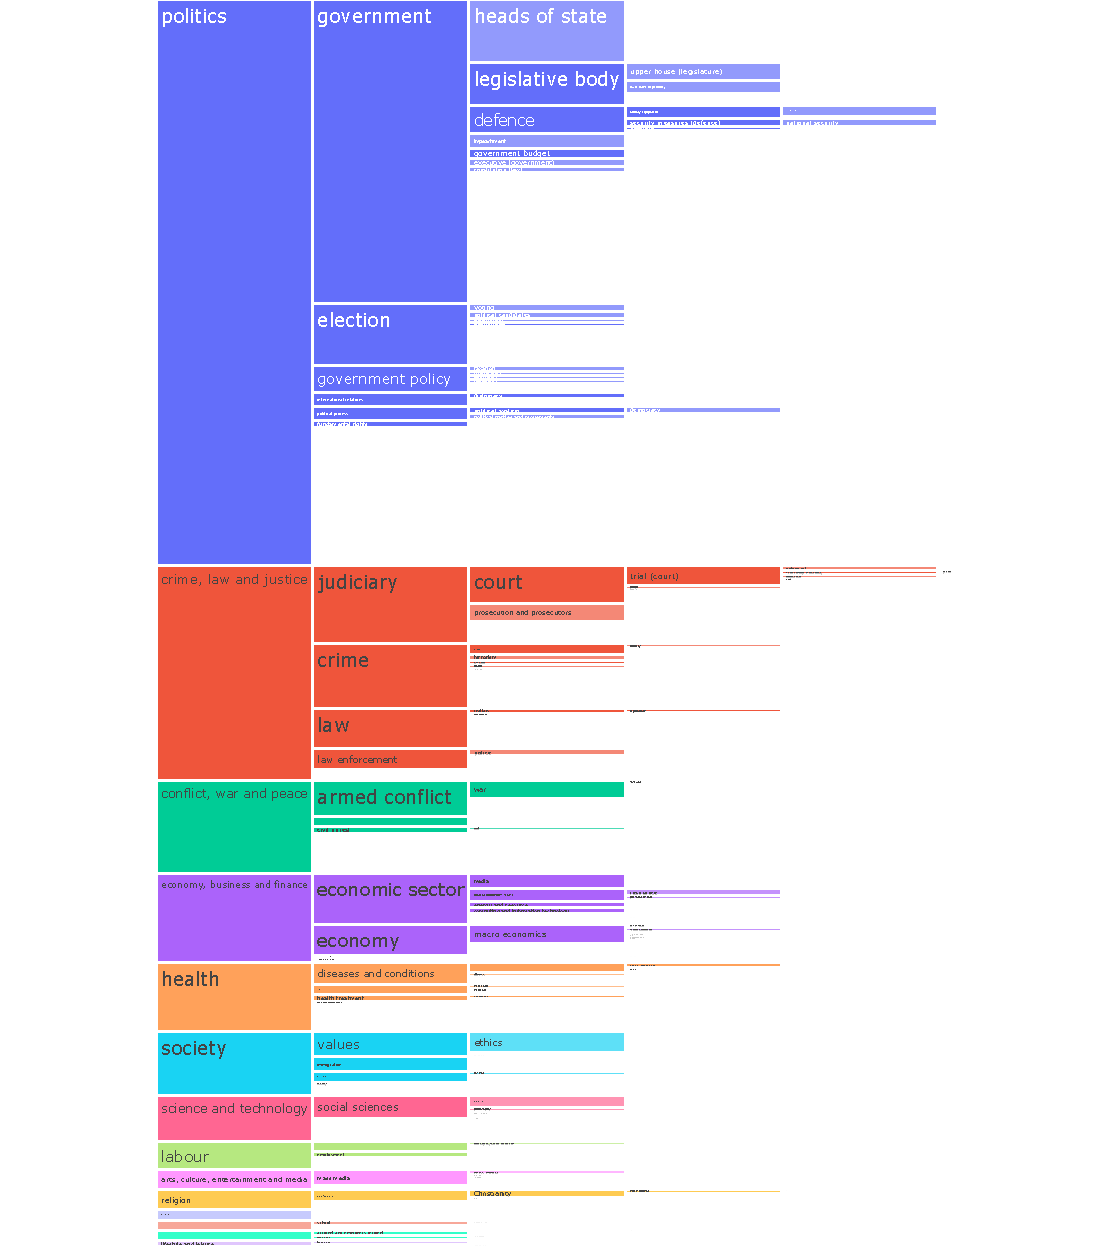
\includegraphics[width=\linewidth]{figures/baly_iptc_weighted.pdf}
    \caption{IPTC topics weighted of \texttt{Baly} dataset}
    \label{fig:baly_iptc_weighted}
\end{figure}


Options:
Multi-topic weighted complex solution
Only see what happens in specific topic with the classifier
Input topics as features and see classifier what produces:
Need to encode the topics hierarchically
Need model (neural network) on top that can combine the features. Single-layer neural network cannot, need 2 layers at least

% \subsection{Results}


\section{Topic analysis across political spectrum}
\label{sec:topics_topics_leaning}
TOPIC+LEANING

Coarse topics are very similar across political spectrum
Fine-grained topics are slightly different (quantity, terms). Which ones? They express the choice of details that we discussed in chapter 3

RQ2: How does the topic (at different granularities) change across political leaning on a parallel news corpus?

\subsection{AllSides topics}

The distribution from the 3 different leanings is very similar. 
Very uneven distribution!!!
Topic merging? How?

\subsection{Coarse Topics}

\subsubsection{Which topics are there (Leaning+Topic)}

TODO FIGURE

The most prominent topics are Politics, Culture, Law and Violence.
Y-axis: the weighted topic count for each article (1=all the articles have the topic, 0=none have the topic)
The distribution of the topics is very similar between the political sides

\subsection{IPTC Topics}
Topics vs leaning: are there topics that are mostly left/right?

TODO FIGURE

Sunburst diagram shows topics that are more left or right (blue=left, red=right)
Topics where there are more articles from:
Left: Election, legislative body, health, science and technology
Right: crime law and justice, government, conflict war and peace, society


\section{Breakdown of propaganda by topics}

This section contains analysis of how propaganda is distributed across topics and what differences topics contain in terms of propaganda.
Assumption: propaganda is used for certain topics more than in others

RQ3: How does the detected propaganda change across the topics?

Experiment 4.3: 
- topic breakdown: AllSides Topics, IPTC
- shapes of propaganda/sentiment 


Types of shapes (propaganda)
(look at purple: propaganda)

Blue is sentiment (+ and -) and purple is propaganda. 
y axis in the fraction of terms marked as sentiment/propaganda.

\subsection{Custom Topics (AllSides)}

How do they overlap with the propaganda techniques?

Every article is tagged with a topic (AllSides) and with the propaganda techniques (from the tool).
We want to see which topics occur with specific propaganda techniques.
For this reason, we build 3 heatmaps (one for each political leaning) with the propaganda techniques on the x-axis and the topics on the y-axis. The value of the cell represents the average quantity of the propaganda technique for that specific topic.
We want to see differences between the Left/Center/Right heatmaps.

TODO FIGURE: HEATMAP? OR WHAT?

Differences:
The Right is using Doubt when talking about “science” far more than the other two political leanings (1.2\% Left - 13 articles, 0.9\% Center - 8 articles, 5.2\% Right - 4 articles). Does this mean that the Right is more sceptical about science? Let’s look at the data (4 articles from the Right with the topic “science”):
https://spectator.org/science-know-it-alls-on-the-march/
http://www.washingtontimes.com/news/2017/apr/22/march-political-science-earth-day-rally-doubles-la/ 
http://www.nationalreview.com/article/447048/bill-nye-science-guy-march-science-left-politics-religion
https://www.foxnews.com/science/we-could-go-to-venus-with-todays-technology-scientists-say 
The first 3 articles cover the 25 April 2017 march for science, which was labelled by some sources on the Right as “the leftist [...] new religion” (nationalreview article)
3 articles compared here: https://www.allsides.com/story/earth-day-march-science 

The Center is using Appeal to Authority when talking about “dea” far more than the other two leanings (0\% Left - 3 articles, 1.8\% Center - 1 article, 0\% Right - 1 article). Does the Center appeal more to authority because it is more “moderate” than Left and Right?
Other cases can be discovered and the classifier can use them (topic+propaganda technique quantity/terms) to recognise political leaning



\subsection{Coarse Topics}

TextRazor has coarseTopics (up to 5 topics for each article, article-level, e.g. Health/Politics/Law/...) and topics (more fine-grained, around 200 for each article). Each coarseTopic and topic has a weight score which is a value between 0 and 1 representing how prominent is that topic in the article.
Idea: topic+propaganda techniques
Which topics are there?
Which topics co-occur most with propaganda?
Observe how L/C/R use each propaganda technique in a specific topic



\subsubsection{Which topics co-occur most with propaganda?}
This is done at the document level.
Co-occurrence: heatmap propaganda techniques and topics

the biggest co-occurrence is between topic violence and technique loaded language.
BUT it’s only a consequence of Violence and Politics occurring more than other topics in the dataset
Solution: for each cell divide by the sum of topic quantity. An article can have multiple topics. The values used for the weighting of the matrices are the same for all the rows.

TODO FIGURE

(each cell is sum(prop\_quantity*topic\_quantity) / sum(topic\_quantity))
Each cell represents the average quantity of each propaganda technique for the articles that have been tagged to that topic (considering the topic weight)


All three political leanings have very similar profiles, with some exceptions





\subsection{Fine-Grained Topics}

Compute for each topic and each leaning, the co-occurrence with each propaganda technique. Then compute the differences (OK with 2 categories, how to do with 3 categories? Variance? But leaning is on a continuum scale), and sort by difference descending → obtain topics with more differences in propaganda quantities
Variance: each observation is the average quantity of propaganda in specific leaning+topic, computed across leaning


:TODO
Then filter and keep only topics with minimum support (to be defined)

How to compare / visualise differences between L/C/R across topics?
Before: heatmaps
Good only for viewing things from the outside, not too fine-grained

What about finding differences by ranking with a function that expresses how much difference is there?
We want topics with high support and have big differences between leaning with respect to a feature (e.g. quantity of a certain technique, term frequencies).

combined\_score = support(topic) * discrepancy

Categorical data comparison?



\subsection{Derived from Entity Types}

entity propaganda feature computation
For each entity, compute the total/average propaganda techniques that co-occur in the same sentence by each political leaning. E.g.: “Donald Trump” used a lot of times with “Doubt” from the Left leaning.

Interesting direction:
With Entity linking (provided by TextRazor) it is possible to find common attributes of the entities that make them targets of Left/Right propaganda. E.g., a category of people as repeated target of Propaganda.

\subsection{IPTC Topics}

Top-level IPTC Topics analysis:
Pretty similar to CoarseTopics plot (using native TextRazor 17 categories):
Politics is the most common top-level topic → But this time we will be able to break it down to subtopics (taxonomy)
Crime and conflict also quite relevant
Topics across L/C/R are quite similar → confirmation, the Baly Dataset comes from triples of articles across political spectrum

Then we can cut the hierarchy in any possible way (e.g. top 2 levels)

Right has more propaganda when talking about politics?
Causal Oversimplification higher values in Right
Still not informative: let’s look at the fine-grained mediatopics

Politics breakdown:
politics>fundamental rights + Loaded Language/Slogans: more in Center
politics>fundamental rights>freedom\_of\_religion + Flag-waving: more in Right
politics>government>espionage and intelligence + Doubt: Right

2nd level mediatopics (not only politics)
Plot is not very clear, but shows (topic-technique associations that differ the most):
Human interest>people shows higher flag-waving in the Left articles
Human interest + name-calling in Left articles
Communities + flag-waving in Right

What all this means:
Specific topics, even if they are covered by both Left and Right, they are treated differently in terms of propaganda techniques
Fine-grained topics as an approximation of similarity
Classifier can probably benefit from the interaction between topics and propaganda

Next:
Refine/quantify differences between political leanings → find more topics with different propaganda usage
Term analysis L/C/R with and without considering propaganda





\section{Topic+leaning+propaganda}

Assumption: propaganda is used for certain topics in a very recognisable way to push for the ideas of the leaning of the source

RQ4: How does the detected propaganda change across topics and leanings? 

\subsubsection{Correlation Left vs Right IPTC}
Exploratory way: observe the correlation between features of the left and features of the right. If correlation is high, it means that the differences are small. Instead if the correlation is low, it means that there exist differences between left and right.


Correlation between L/R of Propaganda quantities (18 values for each article) across topics
The hope is to see that in some subtopics the correlation is low, meaning that the propaganda quantities differ significantly between Left and Right for the subtopic.
On the full dataset, this propaganda feature was not very useful, so let’s see what happens in all the subtopics.

TODO figure

Scale: blue=correlation high, red=correlation low, grey=not computable (all 0)

This is clearly a negative result. This means that the propaganda quantities are not useful at all. Let’s check what happens with other features:


\subsection{Identifying mediatopics with propaganda differences???}

Objective: using mediatopics taxonomy, find the correct level of narrow that shows differences in how propaganda is used but at the same time not to narrow to still have enough articles.

Differences (quantities of propaganda techniques across leanings), but with enough support. For the sorting it would be nice to have a formula like: 
combined\_score = support(topic) * discrepancy
Or just sort by higher discrepancy, with threshold on support(topic)

Discrepancy computed as correlation?
Distribution of propaganda quantities from L and distribution from R
Option 1: links from AllSides to group the articles in triples
Option 2: average in topic ← selected as doesn’t need info that articles A and B are on the same story. Correlation between quantities of each technique in L vs R

\subsection{Testing on coarseTopic}
Correlation of propaganda techniques quantities between L and R, for each coarseTopic. This is to prove/quantify that coarse topics don’t have much difference in propaganda across political leaning

TODO FIGURE

CoarseTopics that have no high correlation:
Mathematics: pearson=-0.0005, spearman=0.60 (GOOD), support is very small [8. 5. 1.] (BAD)
Language: pearson=0.86, spearman=0.93. Support is [ 83.  48. 109.] articles

Pearson vs Spearman: pearson assumes normal distribution, while Spearman no.
Verifying distribution:

Histogram of quantity of Loaded Language (most prominent technique) of Left (blue), Center (pink) and Right (red) in all the articles. It looks like a normal distribution, truncated at the 0. Y-axis=percentage (TOO: should verify mathematically how close to normal distribution)

\subsection{IPTC Media Topics}
Idea:
Find mediaTopics that have differences (Pearson/Spearman below a threshold) and have enough articles for each leaning
Compare distributions of these topics

Politics subtopics with either Pearson or Spearman below 0.9

TODO create table with figure from terminal

Nice to see coming up topics such as religion, censorship, veteran affairs, government.
What instead has high correlations? (=is more similar in quantity of propaganda techniques across L/R) → TODO show/represent on the topic tree the areas that are more similar and more different


\subsubsection{Freedom of Religion}
Let’s take an example, e.g. about Freedom of Religion
9 Articles from the Left, 5 from Center, 21 from Right
politics>fundamental rights>freedom of religion: p= 0.7831403727439277 s= 0.7222989890906132 [ 9.  5. 21.]

Looking at the distributions of these 35 articles:

TODO FIGURE

Flag-waving from Right has more flat distribution (higher average too) than Left
TODO: confusing colors, force to 3 standard colors
TODO: maybe it’s not the best way to compare distributions (something like violin plot)



\section{Leaning classifier: breakdown by topic}

In this section we aim to analyse the relationship between topics, propaganda and leaning from a different perspective.


\section{Predicting Leaning from topics and propaganda}


RQ2: \emph{knowing the topic, does it make classification (prop-->leaning) easier?}

7: topics+propaganda for political leaning prediction


\section{Discussions}


\section{Conclusions}
What is the conclusion of this work?